\chapter{斯特林机组排列方式优化研究}
\label{cha:optSEA}

由\autoref{sec:StirlingEngineModel}中对斯特林机的机理建模研究分析可知,对于单台斯特林机,斯特林机与传热流体之间的换热过程和流体的流动方向无关,这意味着改变冷热流体的流动方向并不会影响斯特林机的功率和效率。然而,本文的梯级系统中考虑了使用多台斯特林机组成斯特林机组。

对于多台斯特林机,斯特林机的连接方式和流体的流动方向需要进行优化分析。它们既影响冷热流体的温度,又影响冷热流体的质量流量分布,这二者对斯特林机的功率和效率都有很大影响。


如果采用串联连接,则一方面,每台斯特林机都可以获得全部的流体流量,这有利于获得较高的输出功率;另一方面,各斯特林机的入口加热流体温度随着流动方向逐渐降低(或各斯特林机的入口冷却流体温度随着流动方向逐渐升高),这将使沿着流动方向的斯特林机的功率和效率逐渐下降。如果采用并联连接,则一方面,每台斯特林机的入口加热流体的温度都为最高值(或每台斯特林机的入口冷却流体的温度都为最低值),这有利于获得较高的输出功率;另一方面,由于每台斯特林机都分流了热流体(或冷流体)的流量,每台斯特林机的输入总能量降低,这将不利于获得较高的输出功率。如果采用顺流连接(这里的顺流和逆流是指冷热流体依次流经一列斯特林机的次序是否一致,和传统的换热器中的顺流和逆流的含义不同),则一方面,最先流经的数台斯特林机具有最大的冷热源温差,具有最大的输出功率;另一方面,最后流经的数台斯特林机具有最小的冷热源温差,具有最小的输出功率。如果采用逆流连接,则会使斯特林机组中的每台斯特林机具有接近的冷热源温差,每台斯特林机的输出功率都比较接近。对于传统的换热器,采用逆流可以降低冷热流体的传热温差,降低换热过程中产生的㶲损,并因此获得更优的换热效果。而对于斯特林机,需要增大冷热流体的温差,以提高斯特林机的输出功率和效率。


为此,分析不同斯特林机组排列方式对斯特林机组性能(包括功率和效率)的影响,并优化梯级系统中斯特林机组的排布,是非常有意义的。

\section{斯特林机组的排列方式}
\label{sec:connectionTypes}
由于斯特林机组的排列方式多种多样,既可以是串联并联,又可以是顺流逆流,还可能是四者的复杂组合。因此在分析斯特林机组的排列方式之前,需要先将其进行归类。

考虑到斯特林机串联并联及流体顺流逆流的可能,除去其它混合的排列方式,则有如\autoref{fig:EightBasicSEA}所示的八种基本排列方式。

\begin{figure}[htbp]
	\centering
	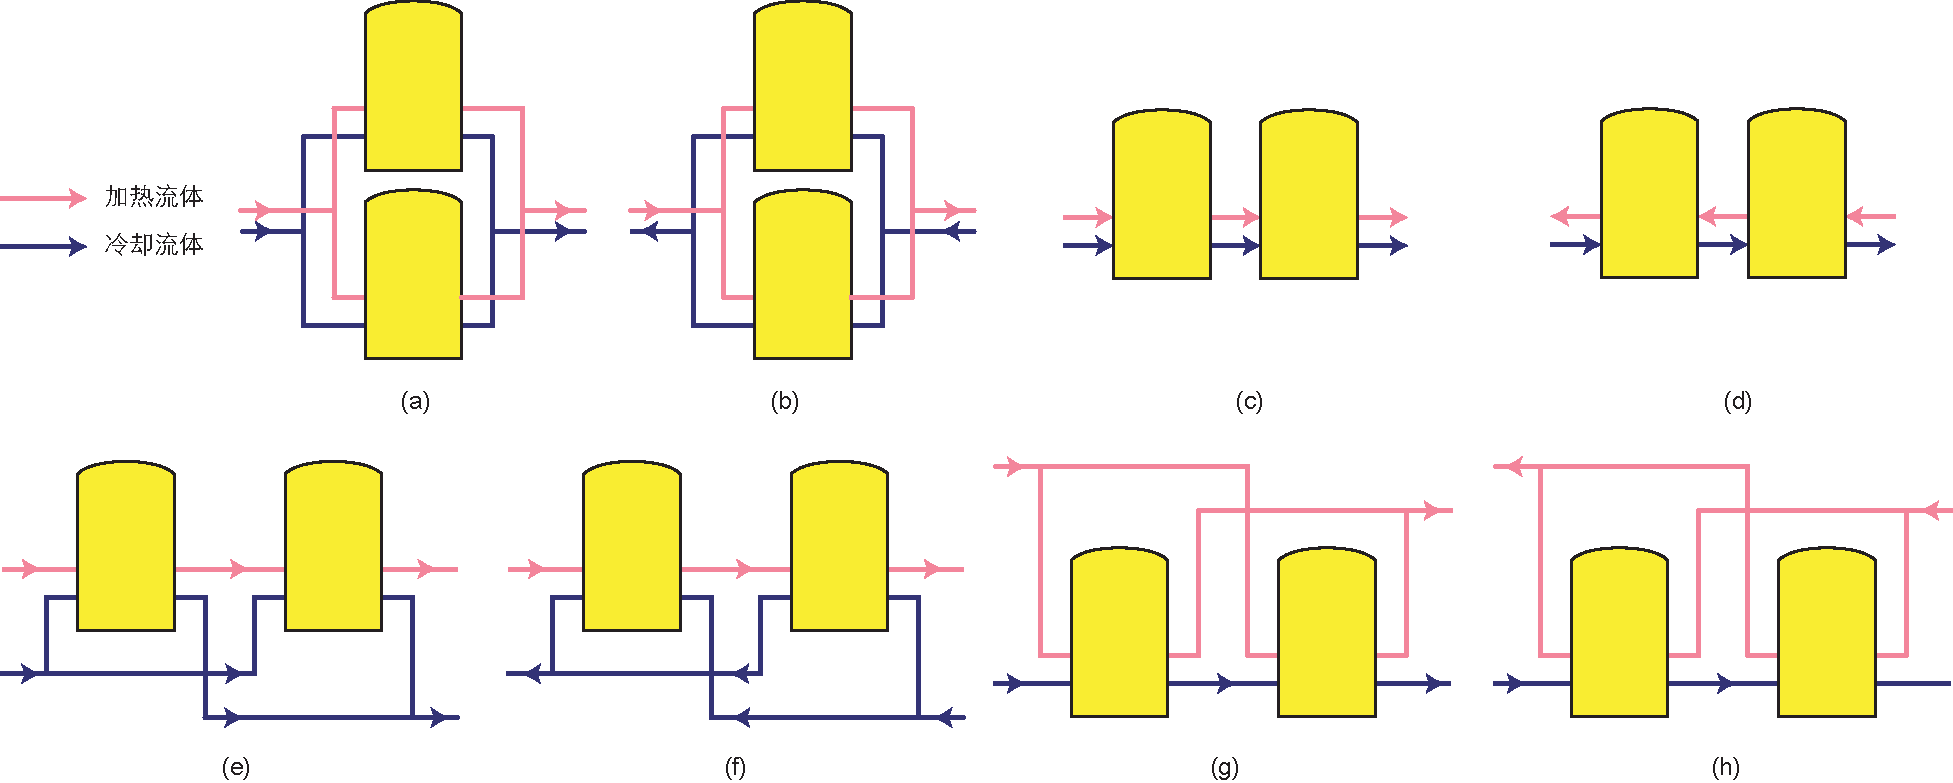
\includegraphics[width = 0.9\columnwidth]{fig/EightBasicSEA}
	\caption{斯特林机组的八种基本连接方式}
	\label{fig:EightBasicSEA}
\end{figure}

本文依据斯特林机的性能与流体流向无关性的特点,将\autoref{fig:EightBasicSEA}中的八种斯特林机组排列方式归纳为如\autoref{fig:SEA}所示的五种基本排列方式,其中,第1种为并联连接,第2种为串联顺流连接,第3种为串联逆流连接,第4种为加热流体串联连接而冷却流体并联连接,第5种为加热流体并联连接而冷却流体串联连接。
这是因为在\autoref{fig:EightBasicSEA}中,排列方式(a)和排列方式(b)的各斯特林机因流经的流体的属性完全相同而具有相同的性能,可以将排列方式(a)和(b)归为\autoref{fig:SEA}中的第1种排列方式。同理,\autoref{fig:EightBasicSEA}中的排列方式(e)和排列方式(f)可以归为\autoref{fig:SEA}中的第4种排列方式;\autoref{fig:EightBasicSEA}中的排列方式(g)和排列方式(h)可以归为\autoref{fig:SEA}中的第5种排列方式。

\begin{figure}[htbp]
\centering
	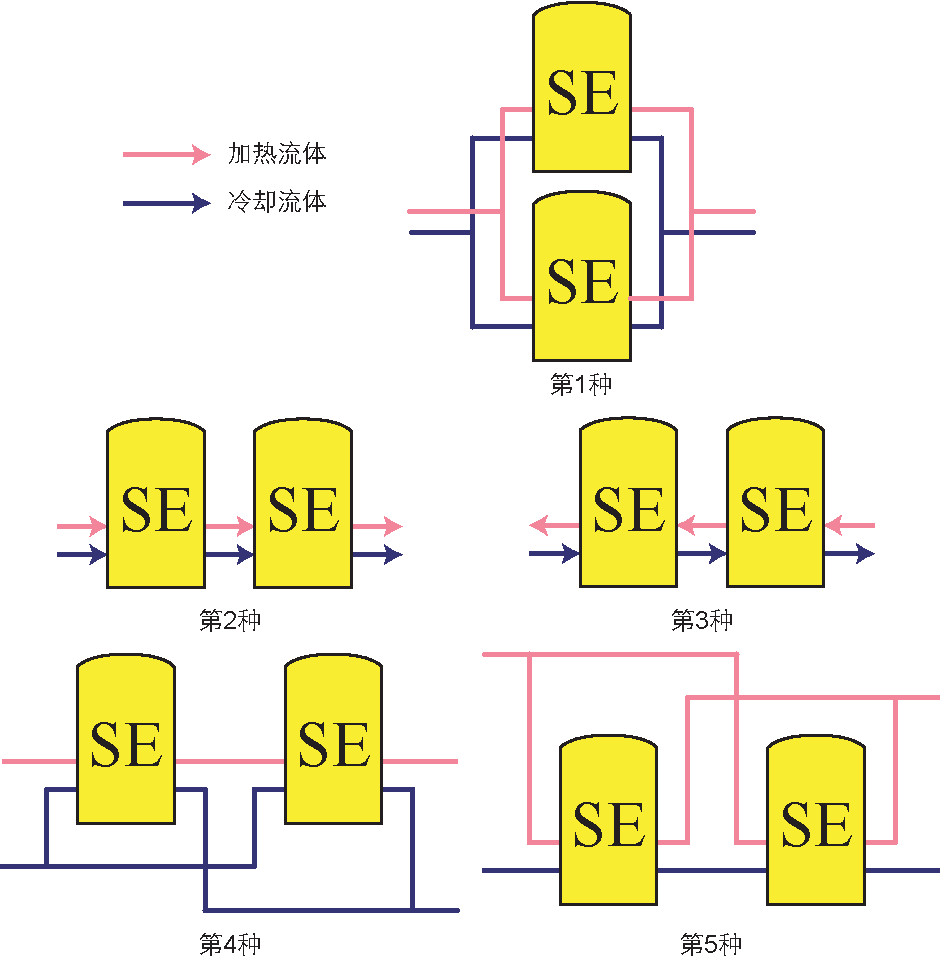
\includegraphics[width = 0.45\columnwidth]{fig/BasicSEA}
	\caption{斯特林机组的五种基本连接方式}
	\label{fig:SEA}
\end{figure}

所有其它的斯特林机组的连接方式都为\autoref{fig:SEA}中的五种基本方式的组合。例如,\autoref{fig:SEA_eg}中斯特林机组的排列方式是第2种和第4种的组合。\autoref{fig:SEA}中的五种排列方式是本文对斯特林机组排列方式的研究基础。

\begin{figure}[htbp]
\centering
	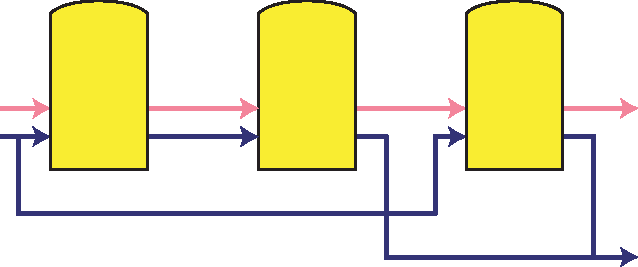
\includegraphics[width = 0.3\columnwidth]{fig/SEA_eg}
	\caption{一种斯特林机组连接方式的例子}
	\label{fig:SEA_eg}
\end{figure}

\section{斯特林机组的建模}

正如\autoref{sec:connectionTypes}中所提到的,存在五种基本的斯特林机组的排列方式,任何其它排列方式是这五种方式的组合。获得了这五种基本排列方式的性能计算方法,就可以计算其它排列方式的性能。

为了得到斯特林机组的性能,需要构建各斯特林机的模型,并依据斯特林机的参数对斯特林机组进行分析。为了便于分析排列方式带来的影响,选定斯特林机组中的各斯特林机具有相同的设计参数,包括转速$s_{se}$。这对于用于发电的斯特林机是个合理的假设,因为各斯特林机的输出功的频率应该保持一致。斯特林机的速度可以通过速度控制系统进行校正\cite{Hooshang2016}。为了消除其它影响,不同排列方式的冷热流体的参数也选择相同值。为了更加清楚地表明排列方式对斯特林机组性能的影响,本文选用换热后温差变化较大的空气作为传热介质。使用空气代替传统的水来给斯特林机冷却,以避免冷却斯特林过程中仅仅产生很小的温升或是导致蒸发带来的一系列不利影响。各斯特林机的设计参数如\autoref{tab:GPU3parameters}所示,斯特林机的其它参数以及冷热流体的参数如\autoref{tab:parameters}所示。如\autoref{sec:modelValidation}中提到的,斯特林机的转速和平均有效压力分别设为25$\,\mathrm{Hz}$和5$\,\mathrm{MPa}$来使所建立的斯特林机模型获得最佳性能预测精度。

\begin{table}[htbp]
\setlength{\abovecaptionskip}{0pt}
	\caption{斯特林机组模型中选用的参数}
	\centering
	\begin{tabular}{cccc}
		\toprule
		参数		&	值	& 参数	&	值\\
		\midrule
		加热流体	&	空气		&	$\dot{m}_h$	&	0.4\,kg/s\\
		冷却流体	&	空气	&	$T_{i,h}$	&	1000\,K\\
		$n_{se}$	&	6	&	$p_{i,h}$	&	5$\times$10$^5$\,Pa\\
		$s_{se}$	&	25\,Hz	&	$\dot{m}_c$	&	0.4\,kg/s\\
		$p_{se}$		&	5\,MPa	&	$T_{i,c}$	&	300\,K\\
		$U_hA_h$	&	180\,W/K	&	$p_{i,c}$	&	5$\times$10$^5$\,Pa\\
		$U_cA_c$		&	180\,W/K	&&\\
		\bottomrule
	\end{tabular}
	\label{tab:parameters}
\end{table}

每台斯特林机组都有两股流体,每股流体都有串联流动和并联流动两种形式,如\autoref{fig:SEA}所示。
对于串联流动,每台斯特林机的流体质量流量均为$\dot{m}$,从流体流动的方向看,对于第$x$台斯特林机($2\leqslant{}x\leqslant{}n_{se}$),
\begin{equation}
	T_{i,x} = T_{o,x-1}
	\label{eq:T_serial}
\end{equation}

对于并联流动,每台斯特林机的流体质量流量均为$\dot{m}/n_{se}$,对于第$x$台斯特林机($2\leqslant{}x\leqslant{}n_{se}$),
\begin{equation}
	T_{i,x} = T_{i,h}
	\label{eq:T_parallel}
\end{equation}

依据\autoref{sec:StirlingEngineModel}中的方程及\autoref{eq:T_serial}到\autoref{eq:T_parallel},已知冷热流体的属性就可以求解各台斯特林机的功率和效率。斯特林机组的功率和效率可以由各斯特林机的功率和热流体的流入流出参数获得。

\begin{equation}
	P_{sea} = \sum_{x = 1}^{n_{se}}P_{se,x}
\end{equation}
\begin{equation}
	\eta_{sea} = \dfrac{P_{sea}}{\dot{m}_1(h_{1o} - h_{1i})}
\end{equation}

系统以MATLAB作为建模工具,利用CoolProp提供的物性参数来进行计算分析,组建斯特林机组的模型。以前文提出的斯特林机参数和流体参数为基础,建立了五种基本斯特林机组排列方式的模型。为了比较各排列方式的性能,以几个参数为变量,研究了不同排列方式下斯特林机组在各种条件下的性能参数。

\begin{figure}[htbp]
\centering
	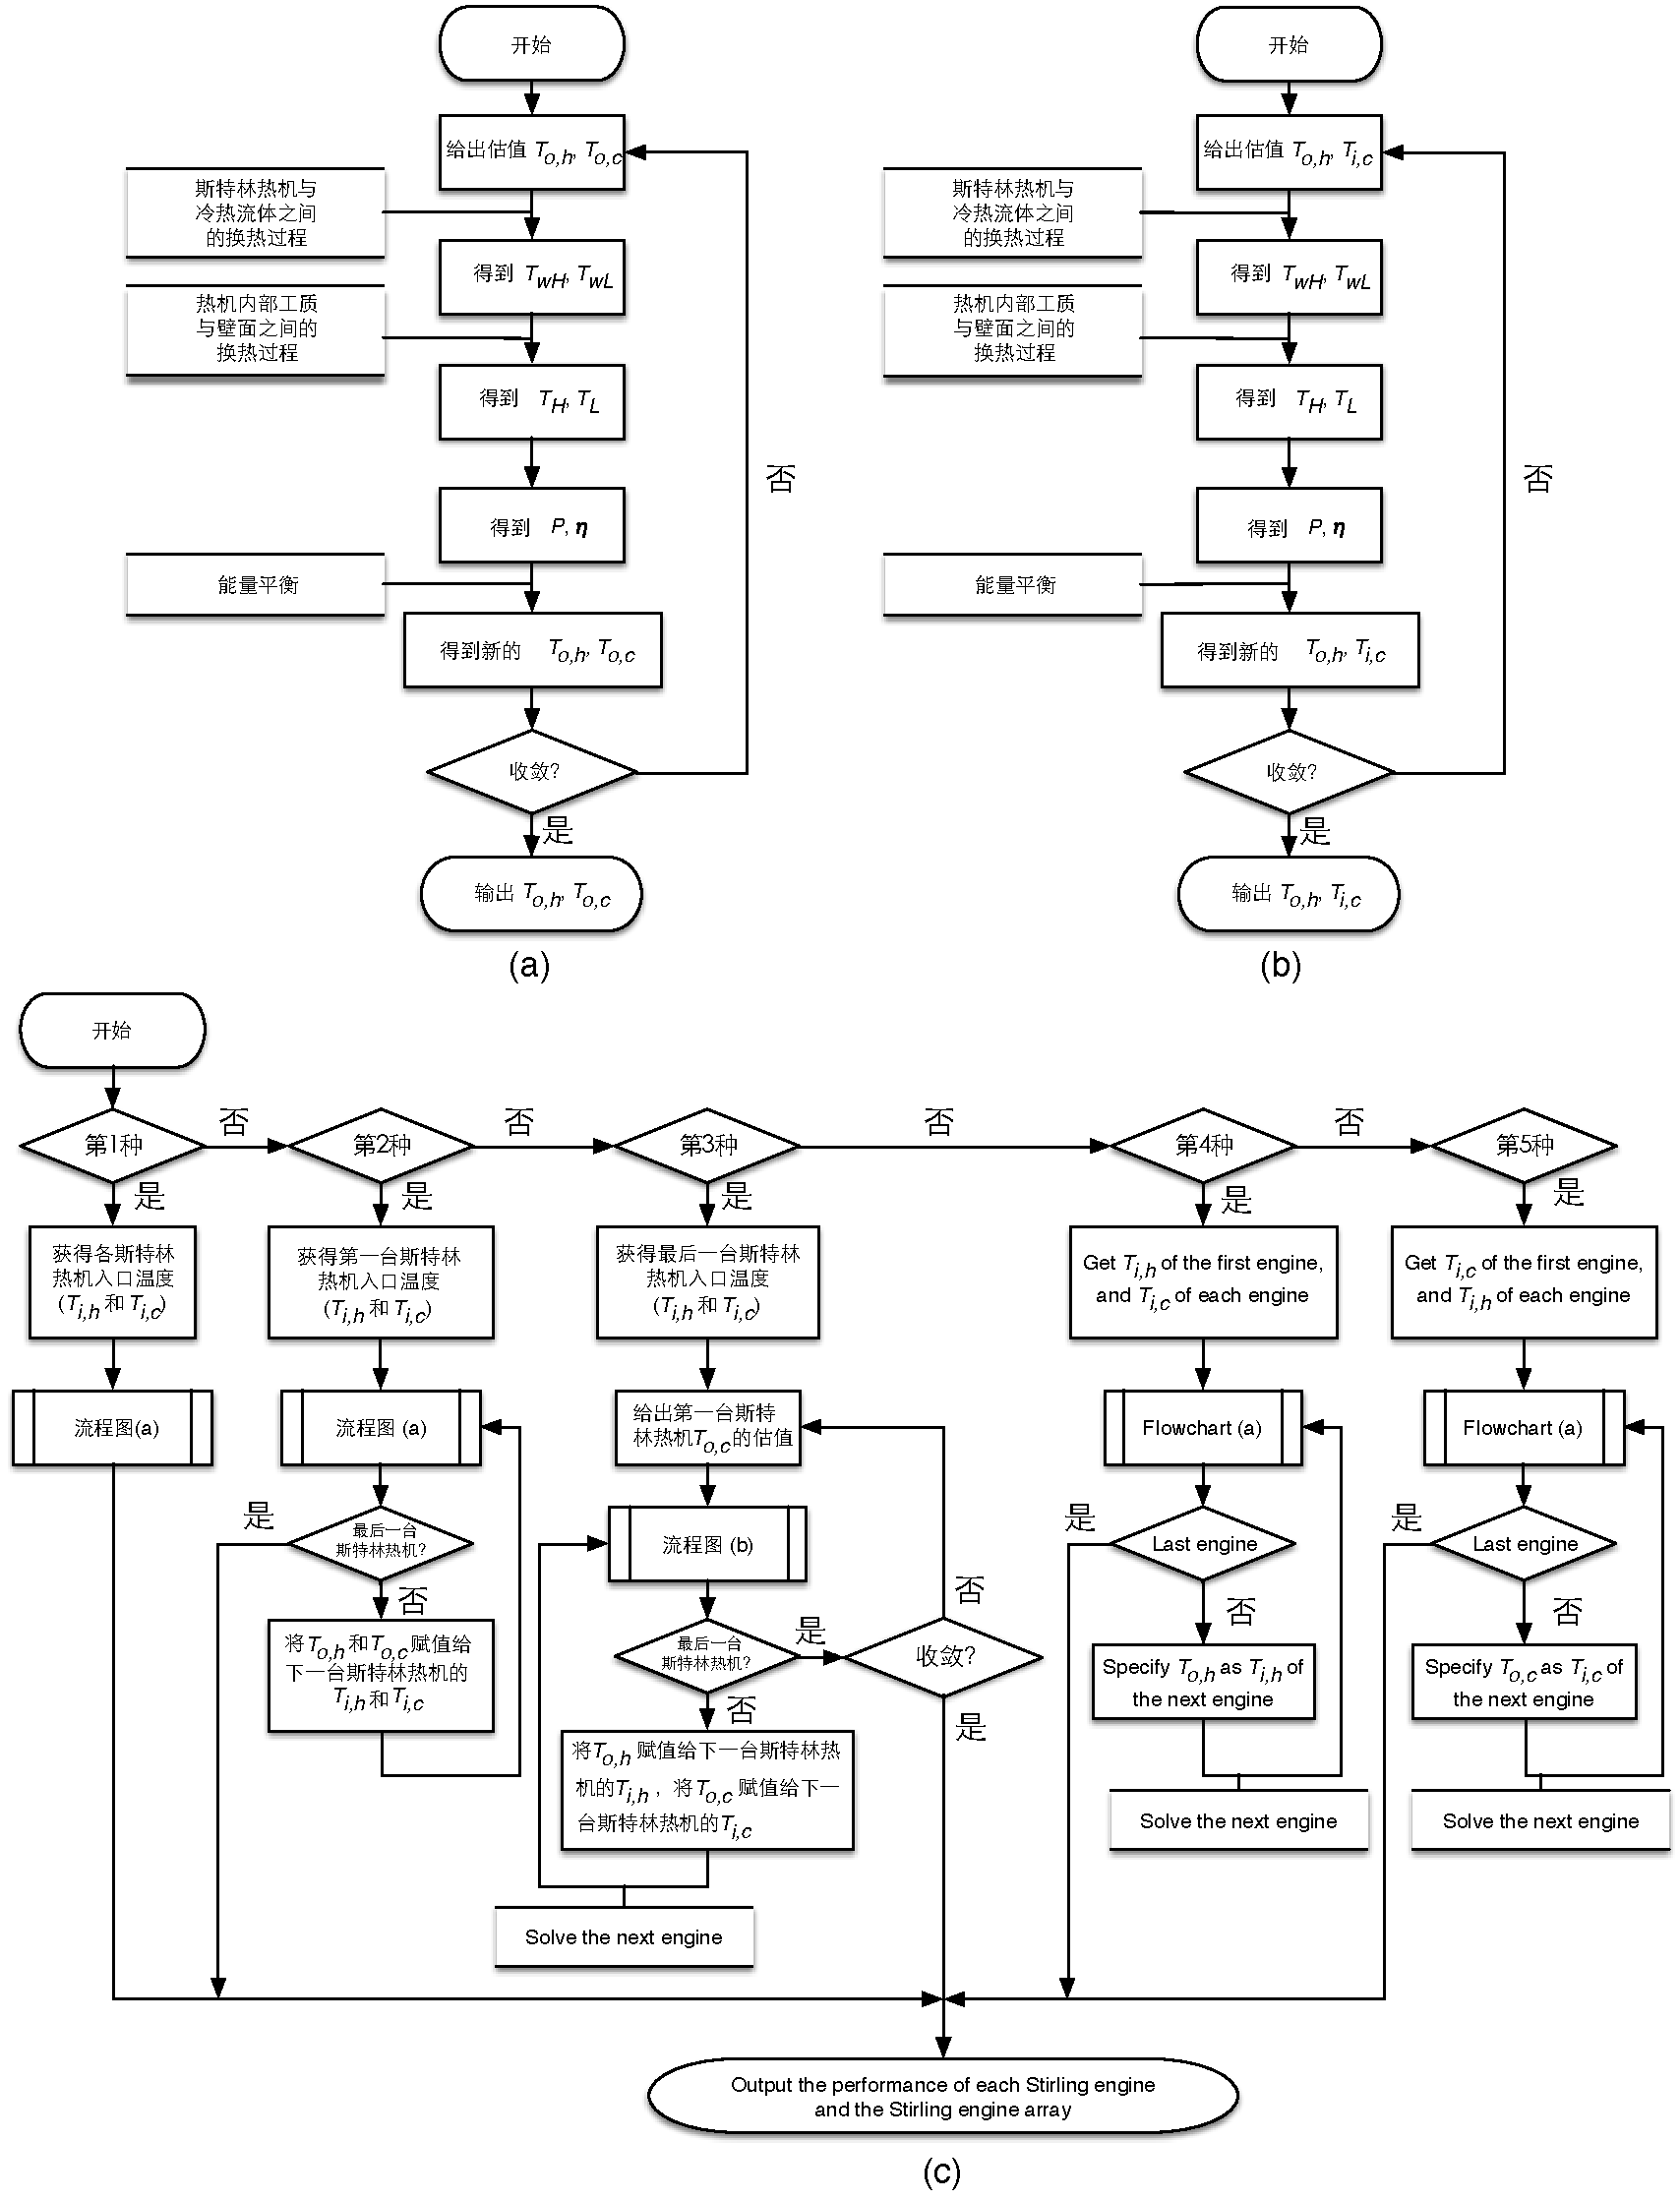
\includegraphics[width = 1.0\columnwidth]{fig/FlowChart}
	\caption{斯特林机组模型的性能分析流程图}
	\label{fig:Flowchart}
\end{figure}

斯特林机组的求解算法如\autoref{fig:Flowchart}所示,其中流程图(a)是求解已知斯特林机入口流体参数(用于顺流)的算法,流程图(b)是求解已知斯特林机热流体入口参数和冷流体出口参数(用于逆流)的算法,流程图(c)是迭代求解各种不同连接方式的求解方法。各流程图中引用了Levenberg-Marquardt算法来求解非线性方程组。

\section{结果分析}
%The objective of this study is to investigate SEA performance difference of different connection types. Therefore, 

本文依据\autoref{tab:parameters}中的参数,建立了不同排列方式的斯特林机组的模型,并依据算法进行了计算分析。各斯特林机组的结果见\autoref{tab:result},其中$\eta_1$,$\eta_2$,$\eta_3$,$\eta_4$,$\eta_5$分别表示第1种排列方式至第5种排列方式对应的斯特林机组的效率;$P_1$,$P_1$,$P_1$,$P_1$,$P_1$分别表示第1种排列方式至第5种排列方式对应的斯特林机组的输出功率。从表中可以发现,在给定的参数条件下,第3种排列方式的斯特林机组具有最高的输出功率和效率,第1种排列方式的斯特林机组中具有最低的输出功率和效率。

\begin{table}[htbp]
\setlength{\abovecaptionskip}{0pt}
	\caption{给定参数条件下不同排列方式的斯特林机组的性能}
	\centering
	\begin{tabular}{p{2cm}<{\centering} p{2.5cm}<{\centering} p{2cm}<{\centering} p{2.5cm}<{\centering}}
		\toprule
		参数		&	值	&	参数		&	值\\
		\midrule
		$\eta_1$	&	0.2215	&	$P_1$		&	8022\,W\\
		$\eta_2$	&	0.2273	&	$P_2$		&	8483\,W\\
		$\eta_3$	&	0.2277	&	$P_3$		&	8512\,W\\
		$\eta_4$	&	0.2227	&	$P_4$		&	8116\,W\\
		$\eta_5$	&	0.2263	&	$P_5$		&	8399\,W\\		
		\bottomrule
	\end{tabular}
	\label{tab:result}
\end{table}

\subsection{热流体入口温度$T_{i,h}$的影响}
\label{sec:T_i_h}
根据\autoref{sec:StirlingEngineModel}中的公式,热流体的温度对斯特林机的效率有很大的影响。斯特林机的效率随着热流体温度的降低而减小。当热流体温度足够低时,热源温度将不足以带动斯特林机,斯特林机的输出功率和效率可能将为零(不工作)。
\begin{figure}[htpb]
\centering
	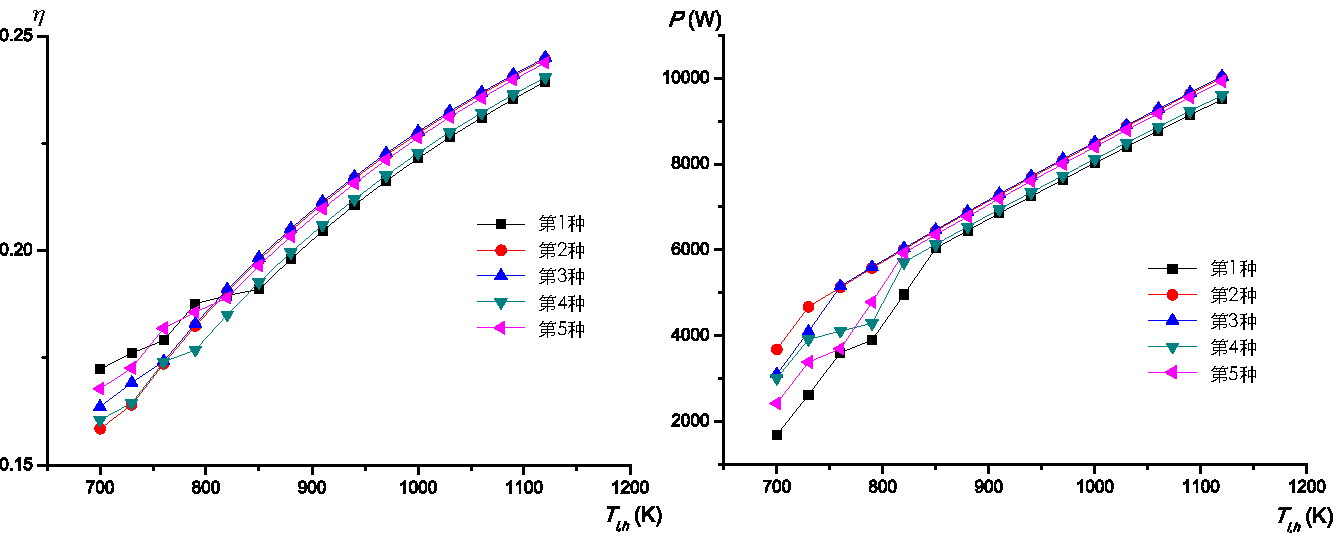
\includegraphics[width = 0.95\columnwidth]{fig/T_ih}
	\caption{入口温度$T_{i,h}$对斯特林机组效率和功率的影响}
	\label{fig:Ti_h}
\end{figure}
斯特林机组对于$T_{i,h}$的性能曲线图如\autoref{fig:Ti_h}所示。随着$T_{i,h}$的增加,所有排列方式的斯特林机组的效率和功率都会上升。然而,对于有些排列方式的斯特林机组,当$T_{i,h}$低于某临界温度时,斯特林机组中的一些斯特林机会停止工作。在这种情况下,适当减少正在运行的斯特林机的数目反而可以增加斯特林机组的总功率输出。当$T_{i,h}$很低时,\autoref{fig:Ti_h}中的一些斯特林机组使用了这种策略。$\eta$-$T_{i,h}$和$P$-$T_{i,h}$曲线上的拐点就是这种策略的结果。图中的数据点都是以在给定的条件下以最大输出功率为目标计算得到的。例如,对于第1种连接方式的斯特林机组,当$T_{i,h} < 850\,\mathrm{K}$时,如果不减少运行的斯特林机数目,则所有斯特林机都会因为较低的热源温度和较小的冷热流体质量流量而停止工作,斯特林机组的输出功率和效率都会降至零。然而,当$T_{i,h} = 820\,\mathrm{K}$时,从6台斯特林机中移除1台斯特林机以后,由于每台斯特林机的冷热流体质量流量都增加了,剩余的5台斯特林机都会再次工作,并获得给定参数下的最大输出功率(虽然效率仍然很低)。$850\,\mathrm{K}$是第1种连接方式的斯特林机组的临界温度,\autoref{fig:Ti_h}中的$\eta$-$T_{i,h}$曲线和$P$-$T_{i,h}$曲线在$850\,\mathrm{K}$处有拐点。

从\autoref{fig:Ti_h}中的曲线可以发现,第2种排列方式和第3种排列方式可以让斯特林机组获得最佳的性能,第2种排列方式具有最佳的健壮性(较低温度下所有斯特林机仍然可以工作)。第2种排列方式中的所有斯特林机在$730\,\mathrm{K}$以上时都会工作。

\subsection{流体热容量$\dot{m}c_p$的影响}

根据\autoref{eq:q_h}和\autoref{eq:q_c},流体热容量$\dot{m}c_p$($\dot{m}_hc_{p,h}$和$\dot{m}_cc_{p,c}$)将会对传热过程产生很大的影响,它是影响斯特林机组性能的一个重要因素。

斯特林机组对于热流体热容量$\dot{m}_hc_{p,h}$的性能曲线图如\autoref{fig:qm_hcp_h}所示。各种排列方式的斯特林机组的性能都随着$\dot{m}_hc_{p,h}$的增加而上升。
对于较大的$\dot{m}_hc_{p,h}$($> 800\,\mathrm{W/K}$),第2种,第3种,第5种排列方式的斯特林机组具有类似的性能,这可以解释为这几种排列方式的冷却流体的属性相同,对于较大的$\dot{m}_hc_{p,h}$,其加热效果在分流后降低地并不明显。同样,当$\dot{m}_hc_{p,h}$较大时,第1种和第4种排列方式的斯特林机组的性能也很接近。这也可以用类似的原因解释。

\begin{figure}[htbp]
\centering
	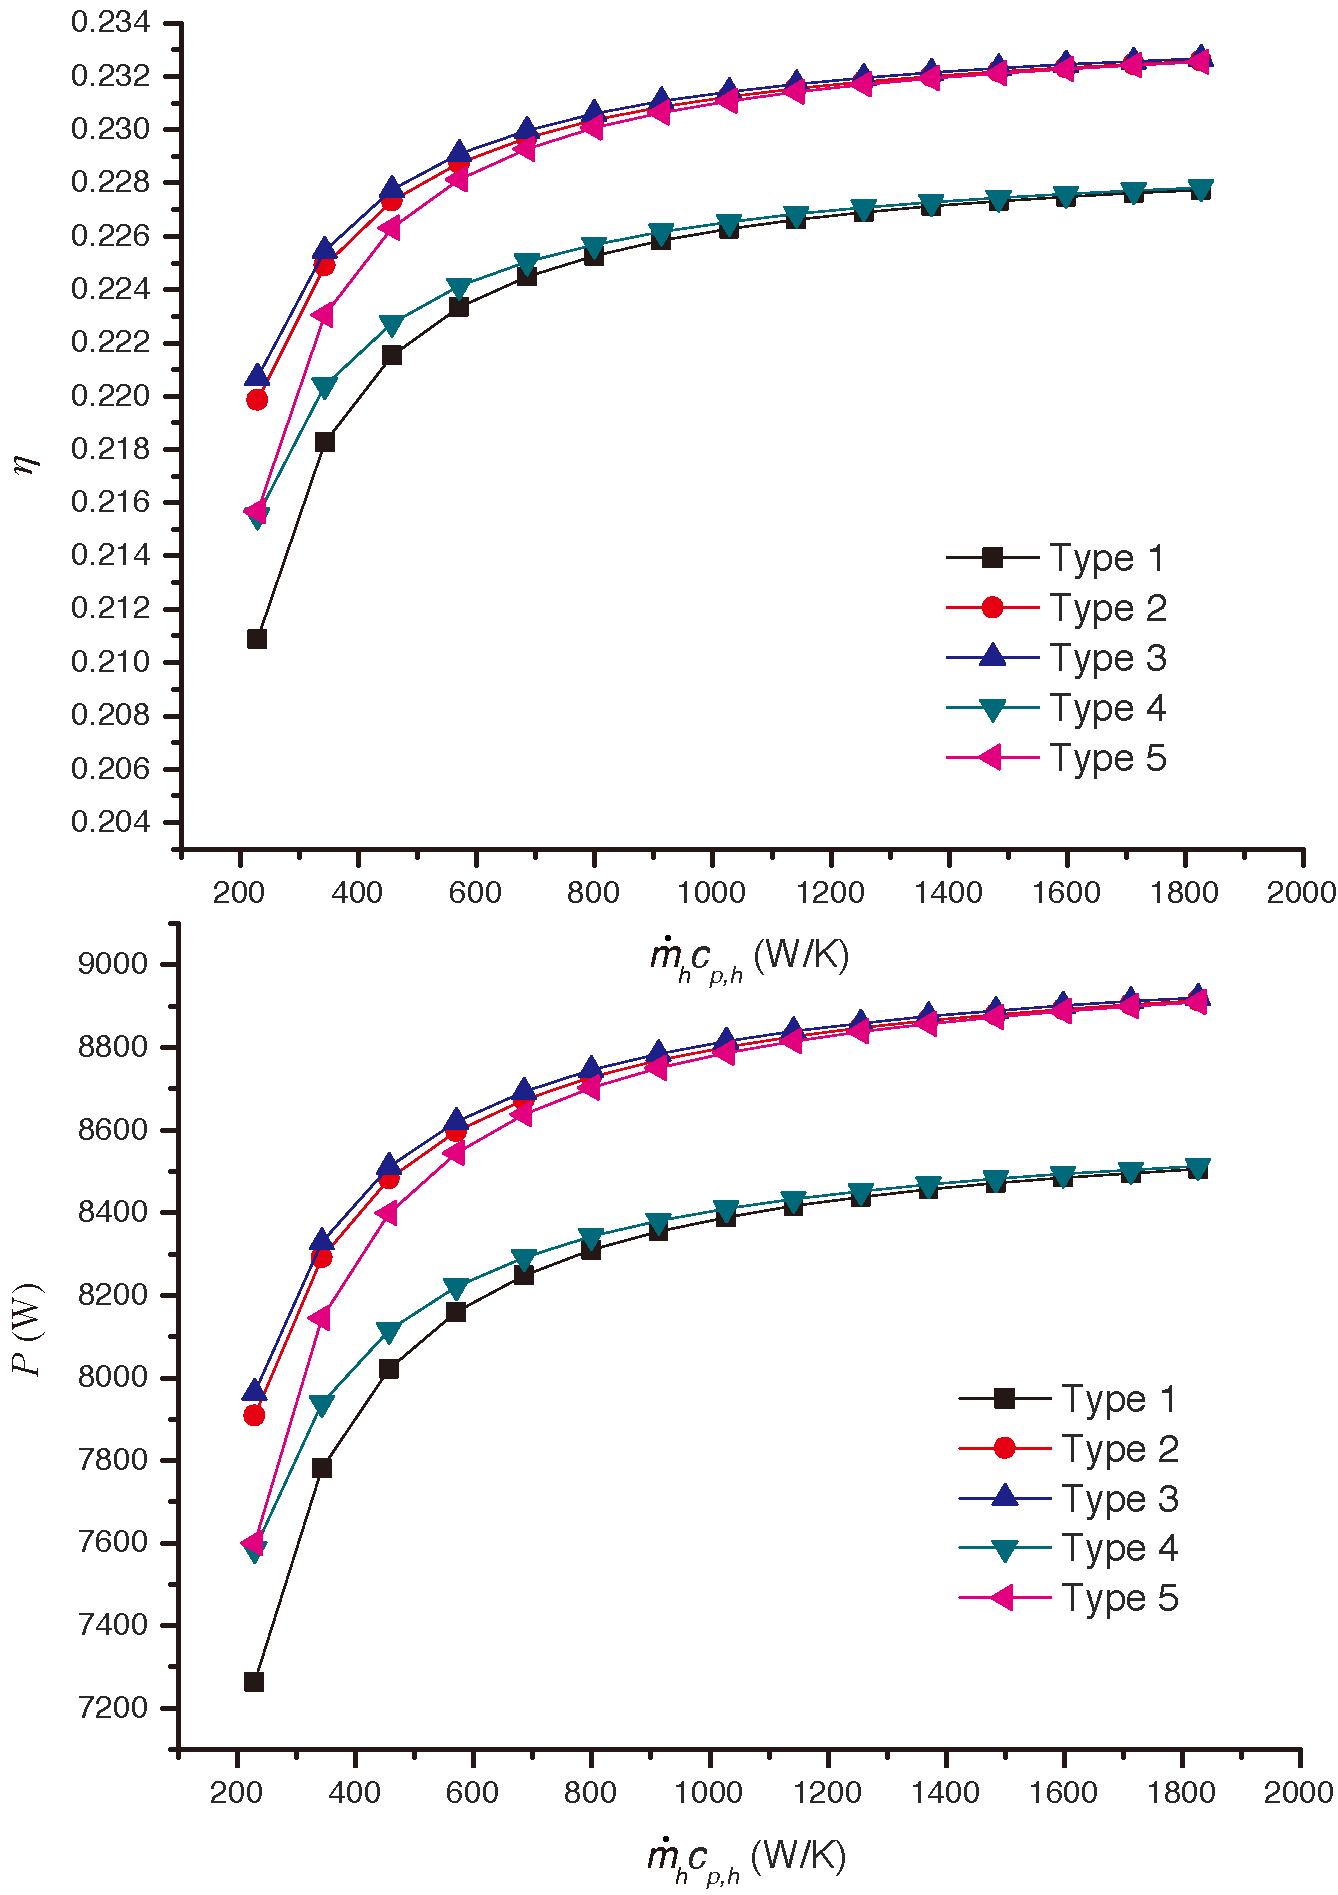
\includegraphics[width = 0.95\columnwidth]{fig/qm_hcp_h}
	\caption{热流体热容量$\dot{m}_hc_{p,h}$对斯特林机组效率和功率的影响}
	\label{fig:qm_hcp_h}
\end{figure}

斯特林机组对于冷流体热容量$\dot{m}_cc_{p,c}$的性能曲线图如\autoref{fig:qm_ccp_c}所示。各种排列方式的斯特林机组的性能都随着$\dot{m}_cc_{p,c}$的增加而上升。
对于较大的$\dot{m}_cc_{p,c}$($> 800\,\mathrm{W/K}$),第2种和第3种排列方式的斯特林机组具有类似的性能,这意味着当$\dot{m}_cc_{p,c}$较大时,顺流或是逆流对斯特林机组的性能的影响不大。第4种和第5种排列方式的性能曲线存在交点(约$830\,\mathrm{W/K}$处),对于较大的$\dot{m}_cc_{p,c}$,第4种排列方式具有更优的性能,对于较小的$\dot{m}_cc_{p,c}$,第5种排列方式具有更优的性能。这可以解释为,较大的$\dot{m}_cc_{p,c}$削弱了冷流体的并行连接带来的不利影响。
\begin{figure}[htbp]
\centering
	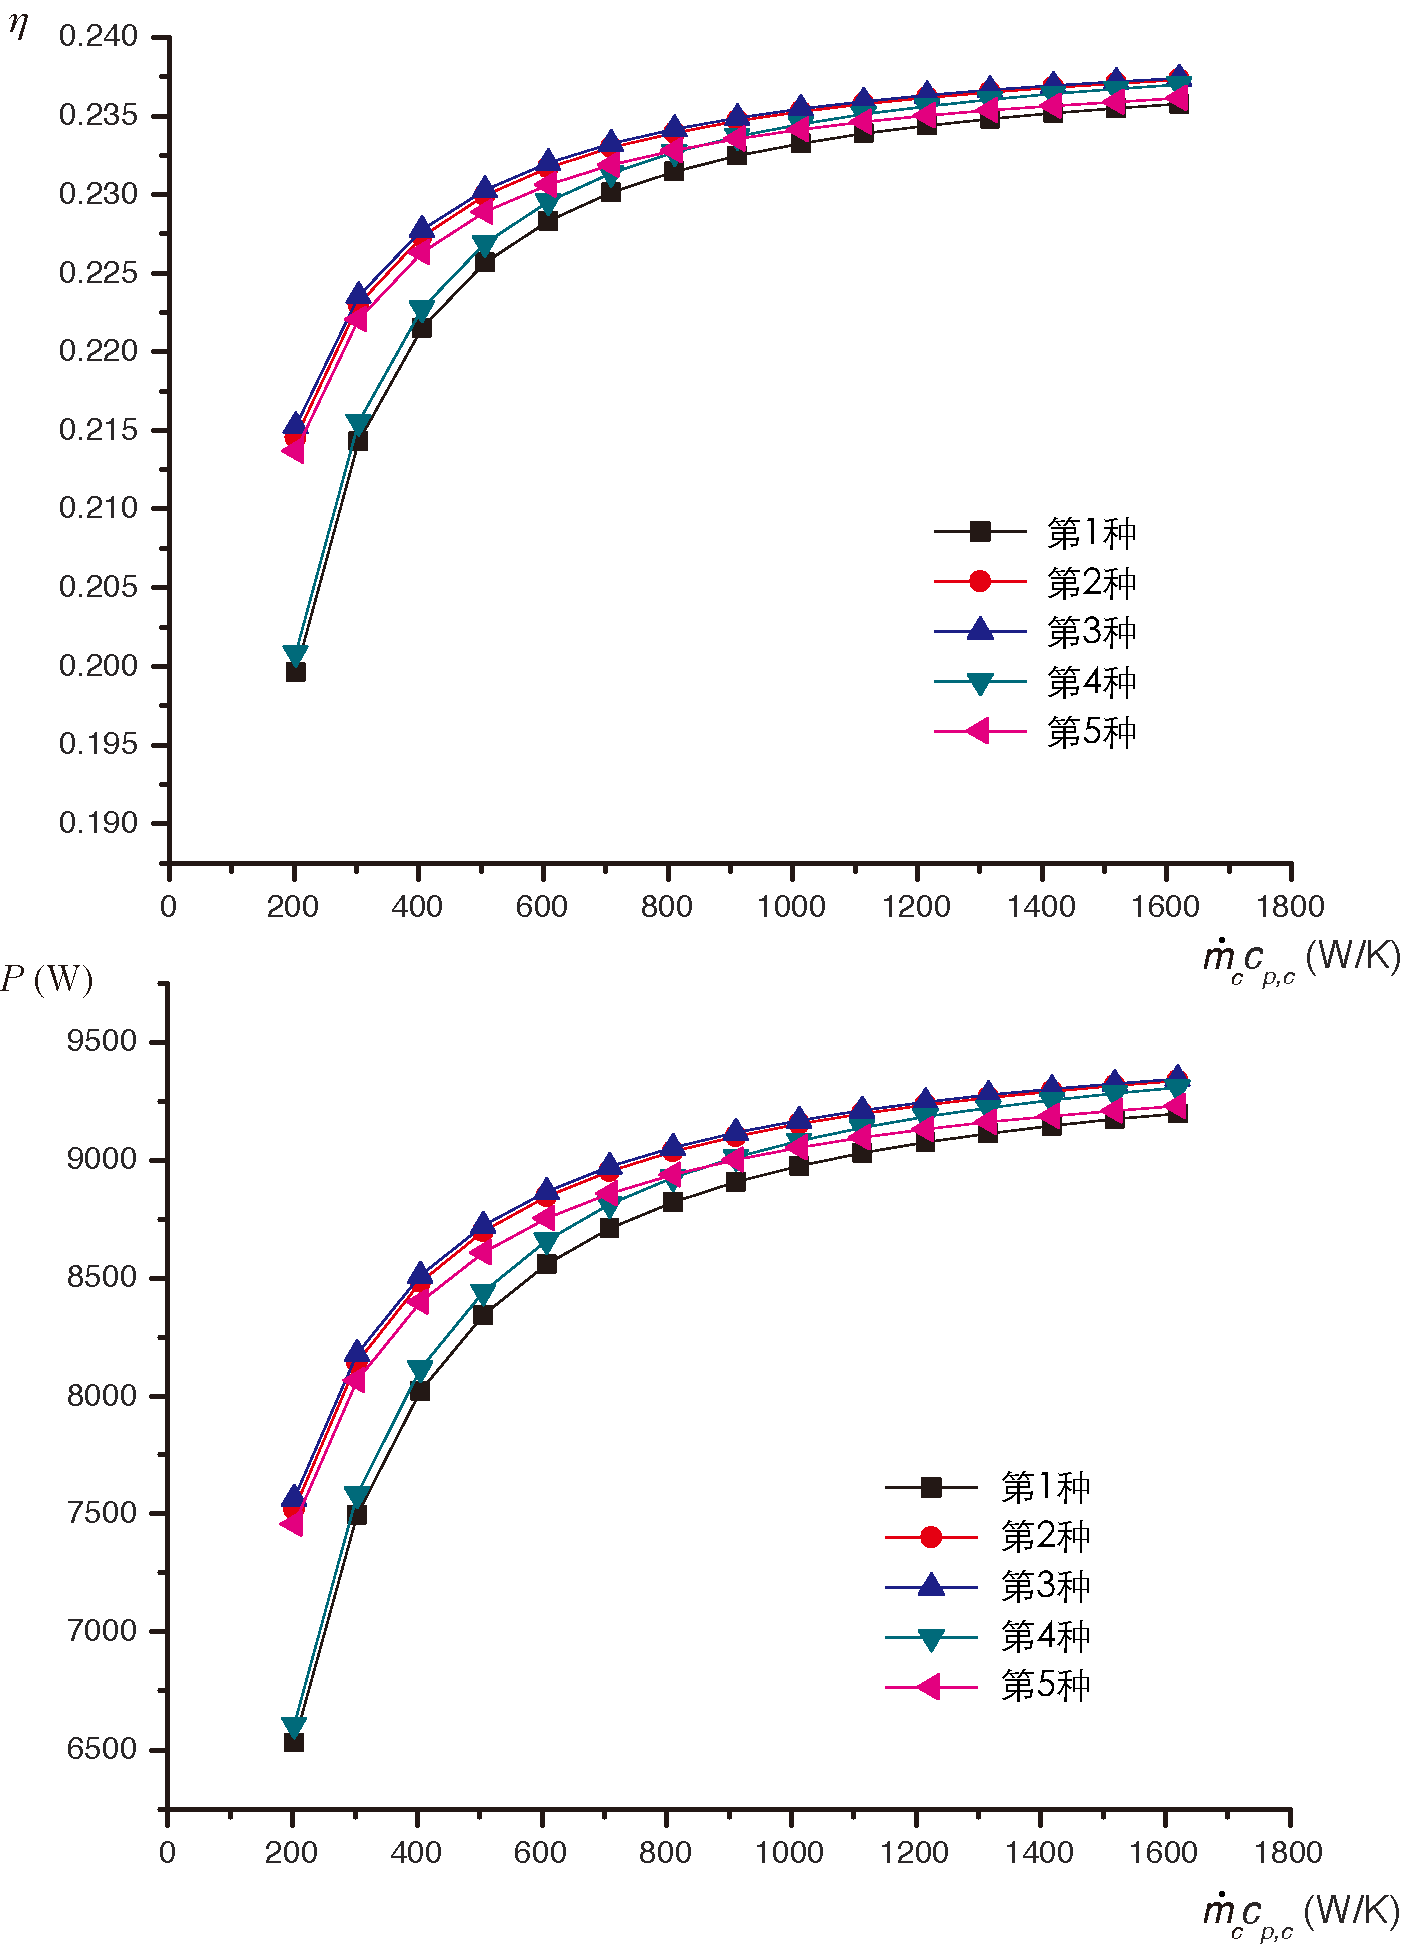
\includegraphics[width = 0.95\columnwidth]{fig/qm_ccp_c}
	\caption{冷流体热容量$\dot{m}_cc_{p,c}$对斯特林机组效率和功率的影响}
	\label{fig:qm_ccp_c}
\end{figure}

\subsection{运行的斯特林机的数目$n_{se}$的影响}

改变运行的斯特林机的数目,斯特林机组的性能也会随之改变。斯特林机的数目$n_{se}$会影响到每一台斯特林机的流体流量和温度。斯特林机组对于$n_{se}$的性能曲线图如\autoref{fig:n_se}所示。随着$n_{se}$的增大,所有排列方式的斯特林机组的效率都会下降。这是由于随着斯特林机数目的增加,每台斯特林机的平均冷热流体温差下降了。对于一些排列方式,$n_{se}$同样存在临界值。当$n_{se}$大于该临界值时,斯特林机组中的一些斯特林机将会停止工作。基于\autoref{sec:T_i_h}所采用的策略,减少运行的斯特林机的数目才能获得最大功率的输出。显然,当$n_{se}$大于临界值时,将运行的斯特林机数目减少至临界值可以获得最大的功率输出。\autoref{fig:n_se}中性能曲线中的水平线部分就是在这种策略下产生的结果。

\begin{figure}[htbp]
	\centering
	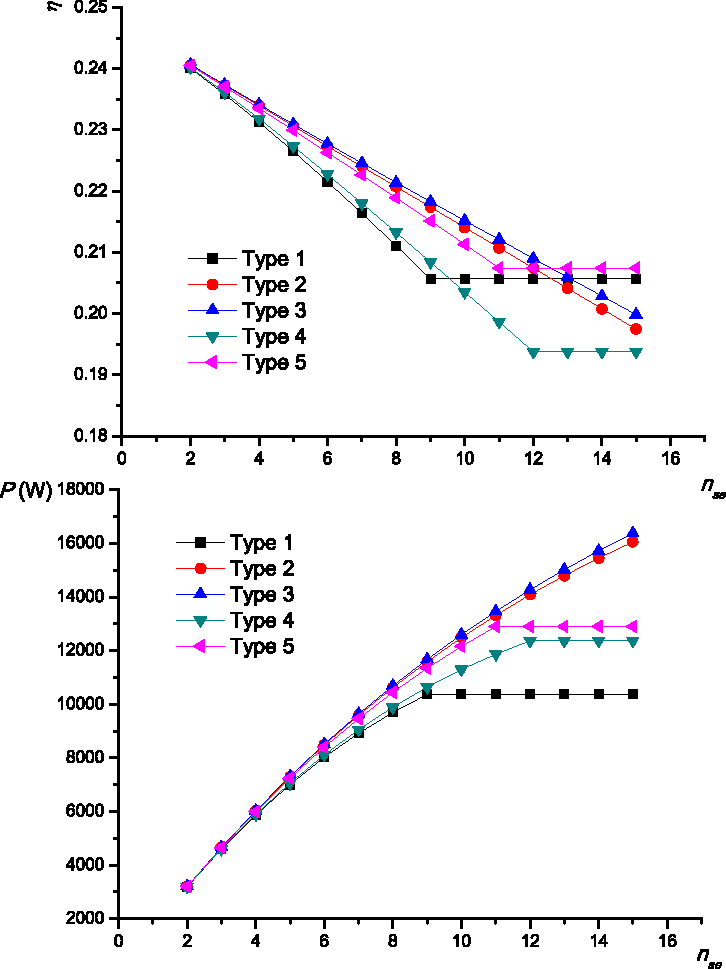
\includegraphics[width = 0.95\columnwidth]{fig/n_se}
	\caption{运行的斯特林机的数目$n_{se}$对斯特林机组效率和功率的影响}
	\label{fig:n_se}
\end{figure}

对于给定的冷热流体,选择合适的斯特林机数目显得格外重要。对于第1种排列方式,当$n_{se} \geqslant 10$时,所有的斯特林机停止工作,这是因为冷热流体的热容量太小。对于第2种和第3种排列方式,所有斯特林机都会工作。斯特林机组的效率随着$n_{se}$的增大而减小,功率随着$n_{se}$的增大而增大。对于第4种排列方式,通过检查计算结果可以发现,如果一直不减少运行的斯特林机数目,当$n_{se} = 13$时,最后1台斯特林机停止工作;当$n_{se} = 14$时,只有前10台斯特林机正常工作;当$n_{se} = 15$时,正常工作的斯特林机数目降至9台。对于第5种排列方式,通过检查结果可以发现,如果不减少运行的斯特林机数目,当$n_{se} = 12$时,最后2台斯特林机停止工作;当$n_{se} = 13$时,只有前8台斯特林机正常工作;当$n_{se} = 14$时,正常工作的斯特林机数目降至6台。

\section{本章小结}

斯特林机组的排列方式影响流体的流量和温度分布,进而影响了斯特林机组中每台斯特林机的性能。为了比较不同排列方式的斯特林机组在不同运行参数下的性能,进而优化太阳能光热发电梯级系统中斯特林机组的排列方式,本文依据斯特林机的特性提出了五种基本的斯特林机组排列方式,并为这五种基本排列方式建立了分析模型。

本章系统性地分析了不同排列方式的斯特林机组在不同$T_{i,h}$、$\dot{m}_hc_{p,h}$、$\dot{m}_cc_{p,c}$及$n_{se}$下的性能,得到了以下结论:

\begin{enumerate}[label=(\arabic*)]
	\item 降低流体入口温度$T_{i,h}$或流体热容量$\dot{m}c_{p}$将会给各种排列方式的斯特林机组的性能带来不利影响。这是显而易见的,因为$T_{i,h}$或$\dot{m}c_p$的降低将导致斯特林机热腔更低的温度分布,斯特林机的热腔和冷腔温差的降低将会削弱斯特林机的性能。
	\item 当热流体的入口温度低于某临界值时,斯特林机组中的一些斯特林机将会停止工作。降低运行的斯特林机的数目则可能会增加斯特林机组的总输出功率。
	\item 不同排列方式对热流体入口温度具有不同的健壮性。第2种排列方式对于较低的$T_{i,h}$具有最佳健壮性,当$T_{i,h} \geqslant 730\,\mathrm{K}$时,所有6台斯特林机都在工作。
	\item 串联排布(第2种和第3种)的斯特林机组具有最优的性能和健壮性。给定了冷热流体,采用串联排布是最优的排列方式。
\end{enumerate}